\documentclass{article}

\usepackage[paperwidth=8.5in,paperheight=11in,left=1.4in,
right=1in,top=1.3in, bottom=1.4in]{geometry}
\usepackage{sectsty, tikz, color, pgfplots}
\usetikzlibrary{shapes,arrows}
\usetikzlibrary{fit}
\makeatletter
\tikzset{
  fn/.style={
    inner sep=0pt,
    fill=none,
    draw=none,
    reset transform,
    fit={(\pgf@pathminx,\pgf@pathminy) (\pgf@pathmaxx,\pgf@pathmaxy)},
  },
  reset transform/.code={\pgftransformreset}
}
\makeatother

    \usetikzlibrary{patterns}
    \tikzset{%
        dotsfill/.style={draw,pattern=dots},
    }

\pgfdeclarepatternformonly[\StripesSize]{MyStripes}{\pgfqpoint{-1pt}{-1pt}}{\pgfqpoint{4pt}{4pt}}{\pgfqpoint{\StripesSize}{\StripesSize}}%
{
  \pgfsetlinewidth{0.3pt}
  \pgfpathmoveto{\pgfqpoint{0pt}{0pt}}
  \pgfpathlineto{\pgfqpoint{3.1pt}{3.1pt}}
  \pgfusepath{stroke}
}

\newdimen\StripesSize
\tikzset{
    StripesSize/.code={\StripesSize=#1},
    StripesSize=3pt
}

\begin{document}
\begin{figure}
  \centering
    \noindent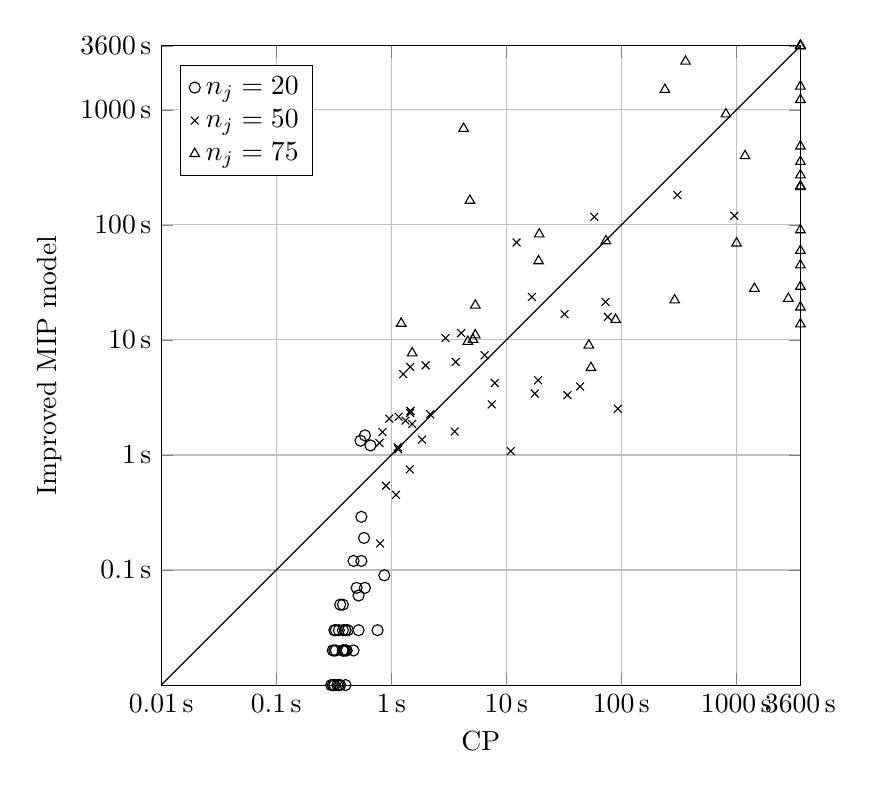
\begin{tikzpicture}

  \begin{loglogaxis}[width=0.8\textwidth, 
  height=0.8\textwidth,xmin=0.01, xmax=3600, ymin=0.01,
  ymax=3600.0,
  xtick = {0.01, 0.1, 1, 10, 100, 1000, 3600},
  xticklabels = {$0.01\,\mathrm{s}$, $0.1\,\mathrm{s}$, $1\,\mathrm{s}$,
  $10\,\mathrm{s}$, $100\,\mathrm{s}$, $1000\,\mathrm{s}$, $3600\,\mathrm{s}$},
  ytick = {0.1, 1, 10, 100, 1000, 3600},
  yticklabels = {$0.1\,\mathrm{s}$, $1\,\mathrm{s}$,
  $10\,\mathrm{s}$, $100\,\mathrm{s}$, $1000\,\mathrm{s}$, $3600\,\mathrm{s}$},
  y tick label style={
        /pgf/number format/.cd,
            fixed,
            fixed zerofill,
            precision=2,
        /tikz/.cd
    }, 
     x tick label style={
        /pgf/number format/.cd,
            fixed,
            fixed zerofill,
            precision=2,
        /tikz/.cd
    }, grid,
    log ticks with fixed point, 
    legend pos = north west,
    xlabel=CP, ylabel=Improved MIP
    model]
\addplot[color=black, mark=o,only marks] coordinates {
(0.47, 0.12)
(0.36, 0.01)
(0.33, 0.02)
(0.87, 0.09)
(0.32, 0.03)
(0.42, 0.03)
(0.35, 0.03)
(0.4, 0.02)
(0.59, 1.48)
(0.32, 0.01)
(0.36, 0.05)
(0.52, 0.06)
(0.59, 0.07)
(0.54, 1.33)
(0.32, 0.02)
(0.76, 0.03)
(0.58, 0.19)
(0.38, 0.05)
(0.39, 0.02)
(0.35, 0.01)
(0.55, 0.12)
(0.34, 0.01)
(0.3, 0.01)
(0.38, 0.02)
(0.47, 0.02)
(0.31, 0.02)
(0.4, 0.03)
(0.31, 0.01)
(0.66, 1.21)
(0.38, 0.02)
(0.38, 0.03)
(0.52, 0.03)
(0.4, 0.03)
(0.33, 0.03)
(0.5, 0.07)
(0.4, 0.01)
(0.55, 0.29)
(0.38, 0.02)
(0.32, 0.01)
(0.41, 0.02)
};
\addlegendentry{$n_j = 20$}

\addplot[color=black, mark=x,only marks] coordinates {
(0.8, 0.17)
(7.94, 4.22)
(3.63, 6.44)
(6.47, 7.36)
(1.46, 5.83)
(4.05, 11.46)
(2.96, 10.38)
(16.67, 23.61)
(18.89, 4.46)
(1.1, 0.45)
(1.85, 1.36)
(3.56, 1.6)
(58.07, 117.45)
(7.47, 2.75)
(0.79, 1.27)
(0.84, 1.58)
(32.08, 16.77)
(2.18, 2.26)
(1.45, 0.75)
(93.18, 2.52)
(1.15, 1.12)
(0.9, 0.54)
(0.96, 2.07)
(17.68, 3.42)
(1.33, 1.99)
(33.96, 3.31)
(1.46, 2.32)
(1.99, 6.01)
(76.25, 15.89)
(12.28, 70.34)
(1.47, 2.41)
(1.14, 1.17)
(958.36, 120.04)
(307.31, 181.82)
(43.81, 3.94)
(72.79, 21.39)
(10.93, 1.08)
(1.52, 1.86)
(1.16, 2.15)
(1.27, 5.04)

};
\addlegendentry{$n_j = 50$}
\addplot[color=black, mark=triangle,only marks] coordinates {
(4.25, 686.76)
(3600, 3600)
(809.75, 917.72)
(54.38, 5.73)
(4.82, 162.87)
(3600, 3600)
(3600, 482.56)
(3600, 29.11)
(3600, 44.66)
(361.32, 2635.11)
(1.52, 7.69)
(73.35, 72.48)
(3600, 1223.32)
(3600, 214.52)
(89.18, 15)
(1434.35, 27.96)
(3600, 90.31)
(3600, 3600)
(3600, 3600)
(5.38, 19.99)
(3600, 354.23)
(52.17, 8.98)
(5.13, 10.07)
(290.48, 22.17)
(3600, 59.67)
(3600, 3600)
(1002.86, 69.26)
(4.63, 9.67)
(3600, 19.25)
(19.34, 83)
(19.07, 48.55)
(238.96, 1497.18)
(3600, 1601.3)
(1188.39, 397.64)
(2825.45, 22.87)
(3600, 13.73)
(3600, 217.45)
(3600, 270.99)
(1.22, 13.89)
(5.37, 11.01)
};
\addlegendentry{$n_j=75$}


\addplot[draw=black] coordinates {(0.01,0.01) (3600, 3600)};

  \end{loglogaxis}
\end{tikzpicture}
   \vspace{0.73em}
\caption{Performance comparison over 40 instances with $n_j=20$ (instances
sorted by average performance)}\label{fig:malapertresultcomp}
\end{figure}
\end{document}
